% 2
%\chapter{準備}
\section{準備}

% 2.1
\subsection{基本的用語}
集合$A$の$k$個の要素からなる部分集合の族を$[A]^k$で表す.グラフとは,$E\subseteq [V]^2$を満たす集合の組$G=(V,E)$のことである.$V$の要素をグラフ$G$の頂点と,$E$の要素を$G$の辺と呼ぶ.頂点$v$と辺$e$に対して,$v\in e$となるとき,$v$は$e$に接続するといい,$e$を$v$の接続辺と呼ぶ.1つの辺に接続する2つの頂点はその辺の端点と呼ぶ.頂点$v$の接続辺で$E$に属すもの全体の集合を$E(v)$で表す.グラフ$G$に辺$\{x,y\}$があるとき,$G$の2つの頂点$x,y$は隣接するといい,互いに他方の隣接点と呼ぶ.$G=(V,E)$と$G'=(V',E')$を2つのグラフとする.その頂点集合の間の全単射$\phi :V\rightarrow V'$で,全ての$x,y\in V$に対して$\{x,y\}\in E\Leftrightarrow \{\phi(x),\phi(y)\}\in E'$を満たすとき$G$と$G'$は同型であるという.$G\cup G'= (V\cup V',E\cup E'),G\cap G'= (V\cap V',E\cap E')$とおく.$G\cap G'=\emptyset$のとき$G$と$G'$は交わらない.$V'\subseteq V$かつ$E'\subseteq E$ならば,$G'$を$G$の部分グラフと呼ぶ.$G'\subseteq G$であり,$G'$が$x,y\in V'$となる辺$\{x,y\}\in E$をすべて含むとき,$G'$は$G$の誘導部分グラフであるという.頂点$v$の次数$d_G(v)$とは,$v$の接続辺の個数$|E(v)|$である.$G$が明らかなときは,$d_G(v)$を単に$d(v)$と記す.次数の最大値$\Delta (G)= \max \{d(v)\mid v\in V\}$を最大次数という.道とは次のように与えられる空でないグラフ$P=(V,E)$のことである.
\begin{align*}
  V & = \{x_0,x_1,\ldots,x_k\},\\
  E & = \{\{x_0,x_1\},\{x_1,x_2\},\ldots,\{x_{k-1},x_k\}\}\\
    & (x_i\neq x_j,0\leq i<j\leq k)
\end{align*}
$U$を任意の頂点(または辺)の集合とするとき,$G+U$は,$G$に$U$に属す頂点とその接続辺をすべて追加して得られるグラフである.$P$が道で,$k\geq 3$のとき,グラフ$C=P+\{\{x_{k-1},x_0\}\}$を閉路と呼ぶ.グラフ$G$に対して,その頂点集合を$V(G)$,辺集合を$E(G)$と記す.頂点の集合$A,B$に対して,$V(P)\cap A=\{x_0\}$かつ$V(P)\cap B=\{x_k\}$となるとき,$P=(x_0\ldots x_k)$を$A$-$B$道と呼ぶ.$A=\{x\},B=\{y\}$のとき,$A$-$B$道を単に$x$-$y$道と呼ぶ.2つの頂点$x,y$の距離$d_G(x,y)$とは,$G$における最短の$x$-$y$道の長さである.

% 2.2
\subsection{木}
グラフ理論において,木とはすべての頂点が連結しており,閉路(サイクル)を持たないグラフを指す.特に,根と呼ばれる頂点を1つ指定した木のことを\textbf{根付き木(rooted tree)}と呼ぶ.特別な注釈がない限り,本論文では木という用語は根付き木を意味するものとし,以降は根付き木を単に木と記述する.

$\Sigma$および$\Lambda$を有限アルファベット,$X$を無限アルファベットとする.ただし,$(\Sigma\cup\Lambda)\cap X=\emptyset$が成り立つものとする.また,頂点集合$V_T$と辺集合$E_T$を持つ木を$T = (V_T, E_T)$とする.$\{u,v\}\in E_T$に対して$u$が$v$より根に近いとき,辺$\{u,v\}$を順序対$(u,v)$で表す.以降,本論文では$(u,v)\in E_T$を$\{u,v\}\in E_T$かつ$u$が$v$より根に近いという意味で用いる.さらに,$(u,v)\in E_T$のとき,頂点$u$を$v$の親,$v$を$u$の子と呼ぶ.また,根ではない次数が1の頂点を葉と呼び,葉に接続する辺または変数を\textbf{葉辺(leaf edge)}と呼ぶ.木の頂点集合$V_T$の各頂点には$\Sigma$に属す記号が,辺集合$E_T$の各辺には$\Lambda$に属す記号がそれぞれラベル付けされているものとする.$\Sigma$に属す記号を頂点ラベル,$\Lambda$に属す記号を辺ラベルと呼ぶ.また,$X$に属す記号を変数ラベルと呼び,各$x \in X$にはランクと呼ばれる1以上の整数が割り当てられていると仮定する.

% 図2.1
\begin{figure}[tb]
  \centering
  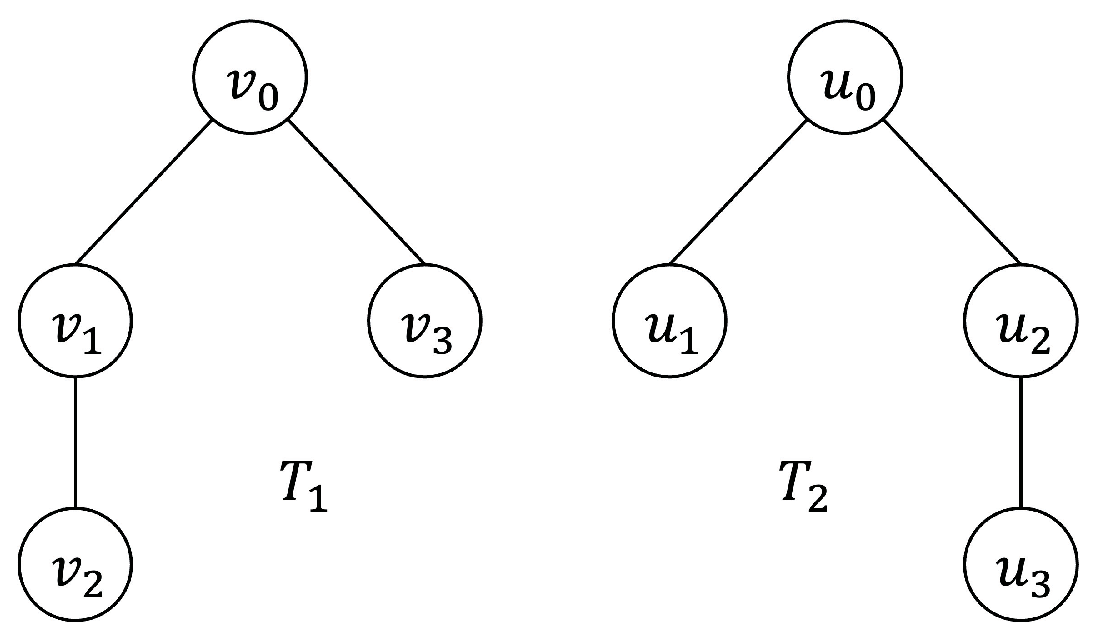
\includegraphics[scale=0.28]{fig/fig-sibling_relationship.eps}
  \caption{$T_1$と$T_2$は,無順序木のときは同型,順序木のときは同型ではない.}\label{fig:sibling_relationship}
\end{figure}

% 2.3
% 無順序木パターン
% 2.3
\subsection{無順序木パターン}
\textbf{無順序木(unordered tree)}とは,後述する順序木と異なり同じ親を持つ頂点に順序関係(兄弟関係)を持たない木のことである.図\ref{fig:sibling_relationship}の2つの木は描き方は異なるが同じ木と扱われる.

% 定義1
\begin{define}{\bf 無順序木における変数}\par
  $\ell$を1以上の整数とする.$T=(V_T,E_T)$の変数とは,次の条件(1)--(3)を満たす$V_T$に含まれる頂点のリスト$h=[v_0,v_1,\ldots,v_{\ell}]$である.
  \begin{enumerate}
    \item[(1)] 頂点$v_0$は子を持つ.
    \item[(2)] $v_1,v_2,\ldots,v_{\ell}$ $(v_i \in V_T, 1\leq i\leq \ell)$は$v_0$の子である.% 順序木のときは「の連続した子である」
    \item[(3)] 変数$h$にはランクが$\ell+1$の変数ラベル$x\in X$がラベル付けされている.
  \end{enumerate}
  $v_0$を変数$h$の親ポート,$v_1,v_2,\ldots,v_{\ell}$を変数$h$の子ポートと呼ぶ.変数の次元とは,その変数に含まれる頂点数のことである.従って,変数$h=[v_0,v_1,\ldots,v_{\ell}]$の次元は$\ell+1$である.\par
  本論文では,変数を図\ref{fig:variable}のように四角で表す.四角に囲まれた文字は変数ラベルを表し,その変数が含む頂点を四角と数字付きの線で結ぶ.数字は変数におけるその頂点の順番を表す.線上の数字は,子ポートの数が1のときは省略する.
  図\ref{fig:variable}では変数ラベル$x$を持つ変数$h=[v_0,v_1,v_2,v_3]$を表す.$h$の次元は4である.
\end{define}

% 図2.2
\begin{figure}[tb]
  \centering
  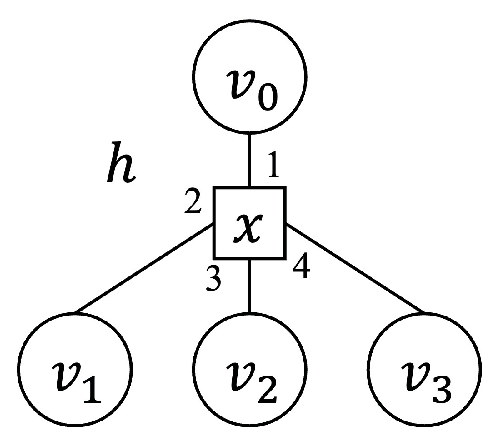
\includegraphics[scale=0.28]{fig-variable.eps}
  \caption{変数ラベル$x$を持つ変数$h=[v_0,v_1,v_2,v_3]$}\label{fig:variable}
\end{figure}

% 定義2
\begin{define}{\bf 無順序項木パターン(unordered term tree pattern)}\par
  $T=(V_T,E_T)$を無順序木とし,$H_T$を$T$の変数の集合とする.ただし,任意の異なる2つの変数$h_1,\,h_2\in H_T$に対して,$h_1$と$h_2$に共通して現れる頂点は高々1つであるとする.無順序項木パターンとは,次の条件(1)--(4)を満たす3つ組$t=(V_t,E_t,H_t)$である:
  \begin{enumerate}
    \item[(1)] $V_t=V_T$,
    \item[(2)] $E_t=E_T\setminus \left(\bigcup_{[v_0,v_1,\ldots,v_{\ell}]\in H_T}\{(v_0,v_i)\in E_T\mid 1\leq i\leq \ell\}\right)$,
    \item[(3)] $H_t=H_T$,
    \item[(4)] $V_t$に属す頂点の頂点ラベル,$E_t$に属す辺の辺ラベルは,それぞれに対応する$V_T$の頂点ラベル,$E_T$の辺ラベルと同じである.
  \end{enumerate}
\end{define}

% 定義2
\begin{define}{\bf 無順序項木パターンの束縛と代入}\par
  $x\in X$をランク$\ell+1$の変数ラベル,$g$を$\ell+1$個以上の頂点を持つ無順序項木パターンとする.$u_0$を$g$の根とし,$u_1,\ldots,u_{\ell}$を$g$の根以外の互いに異なる$\ell$個の頂点とし,$\sigma=[u_0,u_1,\ldots,u_{\ell}]$とする.このとき,形式$x:=[g,\sigma]$を$g$の$\sigma$による$x$への\textbf{束縛(binding)}または単に$x$の束縛という.
  $f=(V_{f},E_{f},H_{f})$を無順序項木パターンとする.ランク$\ell+1$の変数ラベル$x$を持つ変数が$f$に存在するとき,その変数を$h_1,\ldots,h_k$ $(k\geq 0)$とする.束縛$x:=[g,\sigma]$を変数$h_1,\ldots,h_k$に次のように同時に適用して得られる無順序項木パターンを$f\{x:=[g,\sigma]\}$と書く:
  \begin{enumerate}
    \item[(1)] $g_1,\ldots,g_k$を無順序項木パターン$g$と同型な無順序項木パターンとする.
    \item[(2)] 変数$h_j=[v_0^{(j)},v_1^{(j)},\ldots,v_{\ell}^{(j)}]$ $(1\leq j\leq k)$に関して,$H_f$から変数$h_j$を削除し,$g$の頂点$u_0,u_1,\ldots,u_{\ell}$に対応する$g_j$の頂点$u_0^{(j)},u_1^{(j)},\ldots,u_{\ell}^{(j)}$を,この順序で変数$h_j$の頂点$v_0^{(j)},v_1^{(j)},\ldots,v_{\ell}^{(j)}$と同一視する.同一視後の頂点ラベルは,頂点$v_0^{(j)},v_1^{(j)},\ldots,v_{\ell}^{(j)}$の頂点ラベルを継承する.
  \end{enumerate}
  \textbf{代入(substitution)}とは,$x_i\,(1\leq i\leq n)$が$X$の異なる変数ラベルであるような束縛の有限集合$\theta=\{x_1:=[g_1,\sigma_1],\ldots,x_n:=[g_n,\sigma_n]\}$である.
  ただし,$g_{1},\ldots,g_{n}$には変数ラベル$x_1,\ldots,x_n$を持つ変数が現れないと仮定する.
  代入$\theta$による$f$の\textbf{インスタンス(instance)}とは,$f$に対して,$\theta$の全ての束縛$x_i:=[g_i,\sigma_i]$ $(1\leq i\leq n)$を適用して得られる無順序項木パターンである.代入$\theta$による$f$のインスタンスを$f\theta$と書く.

  無順序木(順序木) $T_1$と$T_2$が無順序木(順序木)として同型であるとき,$T_1\equiv T_2$と書く.

  % 図2.3
  \begin{figure}[tb]
    \centering
    \includegraphics[scale=0.28]{fig-lutp.eps}
    \caption{線形無順序木パターン$t$と無順序木$t\theta \equiv T$を示す.無順序木の場合,代入後の$T$と下に示す$T_1,T_2,\ldots ,T_n$は同型である.}\label{fig:lutp} % 無順序木パターン$t$と無順序木$t\theta\equiv T$
  \end{figure}

  $\Sigma,\Lambda$をそれぞれ頂点ラベルの集合,辺ラベルの集合とする無順序木の全体を${\cal UT}_{\Sigma,\Lambda}$とする.また,$\Sigma,\Lambda,X$をそれぞれ頂点ラベルの集合,辺ラベルの集合,変数ラベルの集合とする無順序項木パターンの全体を${\cal UTTP}_{\Sigma,\Lambda,X}$とする.次のように${\cal UTTP}_{\Sigma,\Lambda,X}$の部分集合を定める:
  \begin{align*}
    {\cal LUTTP}_{\Sigma,\Lambda,X} & = \{t=(V_t,E_t,H_t)\in{\cal UTTP}_{\Sigma,\Lambda,X}\mid\\
    & \hspace*{12pt}\forall h_1,\,h_2\in H_t\,(h_1\not= h_2)\mbox{に対して,}\\
    & \hspace*{12pt}\mbox{変数}h_1\mbox{と}h_2\mbox{の変数ラベルは異なる}\},\\
    {\cal LUTP}_{\Sigma,\Lambda,X} & = \{t=(V_t,E_t,H_t)\in{\cal LUTTP}_{\Sigma,\Lambda,X}\mid\\
    & \hspace*{12pt}\forall h\in H_t\mbox{の次元は2であり,かつ}\\
    & \hspace*{12pt}\mbox{$h$の子ポートは葉である}\}.
  \end{align*}
  
  \noindent
  ${\cal LUTTP}_{\Sigma,\Lambda,X}$に属す無順序項木パターンを\textbf{線形無順序項木パターン(linear unordered term tree pattern)}と呼ぶ.また,${\cal LUTP}_{\Sigma,\Lambda,X}$に属す線形無順序項木パターンを\textbf{線形無順序木パターン(linear unordered tree pattern)}と呼ぶ.

  以降,無順序木$T=(V_T,E_T)$を,変数を持たない無順序項木パターン$T=(V_T,E_T,\emptyset)$とみなす.
\end{define}

% 定義4
\begin{define}{\bf 無順序項木パターン言語}\par
  無順序項木パターン$t\in {\cal UTTP}_{\Sigma,\Lambda,X}$に対して,$t$の無順序項木パターン言語$L(t)\subseteq {\cal UT}_{\Sigma,\Lambda}$を次のように定義する:
  $$L(t)=\{t\theta\in {\cal UT}_{\Sigma,\Lambda}\mid \mbox{$\theta$は$t$の変数への任意の代入}\}.$$
  \noindent
  線形無順序木パターン$t$に対して,$T\in L(t)$となる無順序木$T$の例を図\ref{fig:lutp}にあげる.
\end{define}


無順序項木パターン$t$と無順序木$T$に対して,代入$\theta$が存在して$t\theta\equiv T$となるとき,$t$は$T$にマッチするという.
%無順序項木パターン照合問題は次のように定義される決定問題である:
%
%\medskip
%\noindent
%\textbf{無順序項木パターン照合問題}(${\cal MP}$-${\cal UTTP}$)\\
%\textbf{入力}: 無順序項木パターン$t$と無順序木$T$;\\
%\textbf{問題}: $t$は$T$にマッチするか?
%\medskip
%
%上記問題と同様に,無順序項木パターンを線形無順序項木パターンに限定した\textbf{線形無順序項木パターン照合問題}(${\cal MP}$-${\cal LUTTP}$)を定める.無順序項木パターン照合問題は,$t$が線形無順序項木パターンであったとしても,次元4以上の変数が存在すればNP完全である\cite{shoudai-ieice2018}.一方,全ての変数の次元が2であれば,線形無順序項木パターン$t$に対する無順序項木パターン照合問題には入力サイズの多項式時間アルゴリズムが存在する\cite{shoudai-ieice2018}.従って,線形無順序木パターン$t\in{\cal LUTP}_{\Sigma,\Lambda,X}$に対する無順序項木パターン照合問題は入力サイズの多項式時間で計算可能である.
%無順序項木パターンに対する無矛盾性問題を次のように定義する.\par
%
%\medskip
%\noindent
%\textbf{無順序項木パターンに対する無矛盾性問題}(${\cal CP}$-${\cal UTTP}$)\\
%\textbf{入力}: 無順序木の有限集合$S_+\subseteq {\cal UT}_{\Sigma,\Lambda}$と$S_-\subseteq {\cal UT}_{\Sigma,\Lambda}$,ただし$S_+\cap S_-=\emptyset$.\\
%\textbf{問題}: $S_+\subseteq L(t)$かつ$S_-\cap L(t)=\emptyset$を満たす無順序項木パターン$t\in {\cal UTTP}_{\Sigma,\Lambda,X}$は存在するか?
%\medskip
%
%上記問題と同様に,無順序項木パターンを線形無順序項木パターンに限定した\textbf{線形無順序項木パターンに対する無矛盾性問題}(${\cal CP}$-${\cal LUTTP}$)を定める.Miyanoら\cite{miyano-ngc2000}は正規パターンに対して定義された無矛盾性問題がNP完全であることを示した.その結果から,${\cal CP}$-${\cal LUTTP}$がNP完全であることが導かれる.

% 定義5
\begin{define}{\bf 左深さ優先木}\par
  順序木において,左側の子を優先して深さ優先探索を行い,訪れた頂点の深さを並べた整数列を\textbf{深さ列(Depth Sequence)}と呼ぶ.順序木$T$における深さ列は$DS(T)$で表す.この深さ列は,木の構造における頂点の探索順序とその深さに基づいており,深さ優先探索における頂点訪問の順番を整数列として記録したものである.

  一方,無順序木の場合,子の順序が決まっていないため,子の順序を入れ替えることによって異なる順序木を構成することが可能である.無順序木においては,それと同型な様々な順序木表現が構成されるが,その中でも深さ列として辞書式順序で最大の値を持つものを\textbf{左深さ優先木(left depth first search tree)}と呼ぶ.この左深さ優先木がその無順序木を代表する順序木表現と考え,これを\textbf{左深さ優先無順序木(left depth first search unordered tree)}とする(図\ref{fig:left_dfs}).%左深さ優先木は,深さ優先探索において左側の子を優先的に探索するという特性を持つ.
  %具体的には,2つの無順序木が同型である場合,それらの左深さ優先木の深さ列は等しくなる.これは、無順序木の構造においてどのように子の順序を選んでも,左深さ優先木が持つ深さ列が唯一であることを意味している.
\end{define}

% 図2.4
\begin{figure*}[tb]
  \centering
  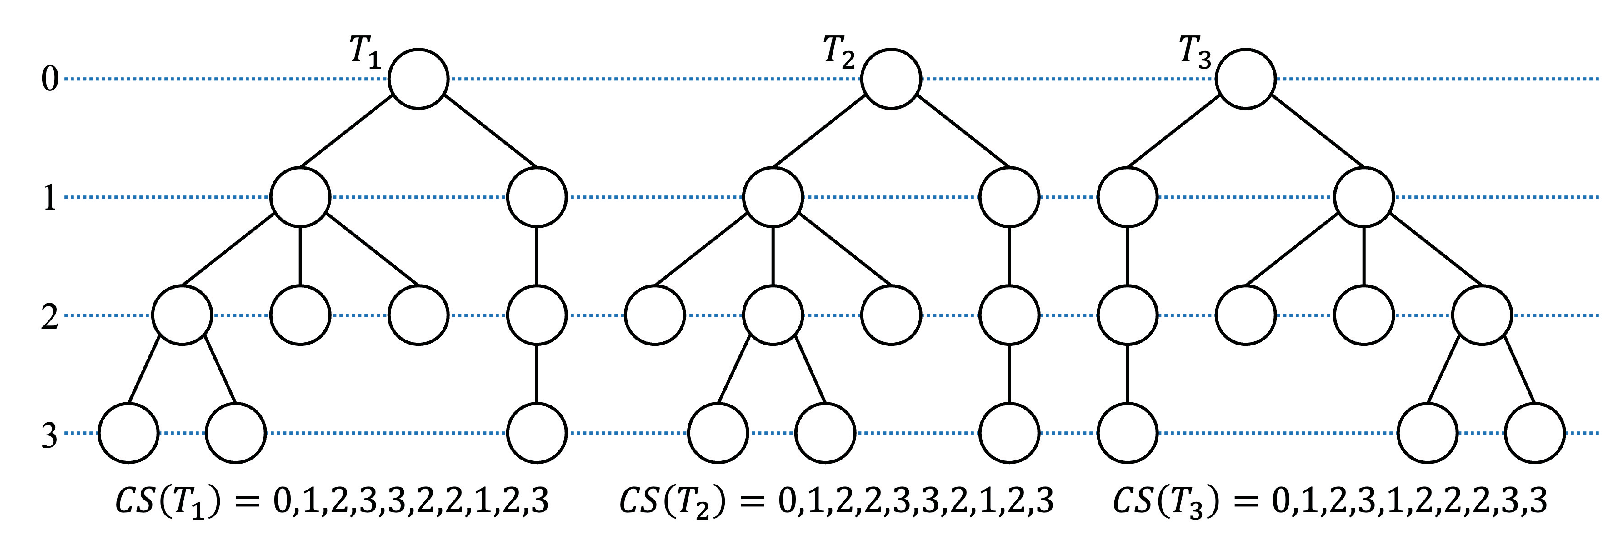
\includegraphics[scale=0.5]{fig/fig-left_dfs.eps}
  \caption{$T_1,T_2,T_3$は同型の無順序木で,左深さ優先木を定めると$T_1$に一意に定まる.}\label{fig:left_dfs}
\end{figure*}

% 2.4
% 順序木
%% 2.4
\section{順序項木パターン}
\textbf{順序木(ordered tree)}とは,同じ親を持つ頂点に順序関係(兄弟関係)を持つ木のことである.順序木の例を図\ref{fig:sibling_relationship}に示す.これらの木は異なる木として扱われる.

% 定義6
\begin{define}{\bf 順序木における変数}\par
  $\ell$を1以上の整数とする.$T=(V_T,E_T)$を順序木とする.順序木$T$の変数とは,次の条件(1)--(3)を満たす$V_T$に含まれる頂点のリスト$h=[v_0,v_1,\ldots,v_{\ell}]$である.
  \begin{enumerate}
    \item[(1)] 頂点$v_0$は子を持つ.
    \item[(2)] $v_1,v_2,\ldots,v_{\ell}$ $(v_i \in V_T, 1\leq i\leq \ell)$は$v_0$の連続した子である.
    \item[(3)] 変数$h$にはランクが$\ell+1$の変数ラベル$x\in X$がラベル付けされている.
  \end{enumerate}
  無順序木における変数と同様に,$v_0$を変数$h$の親ポート,$v_1,v_2,\ldots,v_{\ell}$を変数$h$の子ポートと呼び,変数$h=[v_0,v_1,\ldots,v_{\ell}]$の次元を$\ell+1$とする.
\end{define}

% 定義7
\begin{define}{\bf 順序項木パターン(ordered term tree pattern)}\par
$T=(V_T,E_T)$を順序木とし,$H_T$を$T$の変数の集合とする.ただし,任意の異なる2つの変数$h_1,\,h_2\in H_T$に対して,$h_1$と$h_2$に共通して現れる頂点は高々1つであるとする.順序項木パターンとは,次の条件(1)--(4)を満たす3つ組$t=(V_t,E_t,H_t)$である:
\begin{enumerate}
  \item[(1)] $V_t=V_T$,
  \item[(2)] $E_t=E_T\setminus \left(\bigcup_{[v_0,v_1,\ldots,v_{\ell}]\in H_T}\{(v_0,v_i)\in E_T\mid 1\leq i\leq \ell\}\right)$,
  \item[(3)] $H_t=H_T$,
  \item[(4)] $V_t$に属す頂点の頂点ラベル,$E_t$に属す辺の辺ラベルは,それぞれに対応する$V_T$の頂点ラベル,$E_T$の辺ラベルと同じである.
\end{enumerate}
\end{define}

% 定義8
\begin{define}{\bf 順序項木パターンの束縛と代入}\par
  $x\in X$をランク$\ell+1$の変数ラベル,$g$を$\ell+1$個以上の頂点を持つ順序項木パターンとする.また,$u_0$を$g$の根とし,$u_1,\ldots,u_{\ell}$を$g$の根以外の互いに異なる$\ell$個の葉で,$u_i$が$u_{i+1}$ $(1\leq i\leq \ell-1)$より左の葉であるとき,$\sigma=[u_0,u_1,\ldots,u_{\ell}]$とする.このとき,形式$x:=[g,\sigma]$を$x$の\textbf{束縛(binding)}という.
  $f=(V_{f},E_{f},H_{f})$を順序項木パターンとする.ランク$\ell+1$の変数ラベル$x$を持つ変数が$f$に存在するとき,その変数を$h_1,\ldots,h_k$ $(k\geq 0)$とする.束縛$x:=[g,\sigma]$を変数$h_1,\ldots,h_k$に次のように同時に適用して得られる順序項木パターンを$f\{x:=[g,\sigma]\}$と書く:
  \begin{enumerate}
    \item[(1)] $g_1,\ldots,g_k$を順序項木パターン$g$と同型な順序項木パターンとする.
    \item[(2)] 変数$h_j=[v_0^{(j)},v_1^{(j)},\ldots,v_{\ell}^{(j)}]$ $(1\leq j\leq k)$に関して,$H_f$から変数$h_j$を削除し,$g$の頂点$u_0,u_1,\ldots,u_{\ell}$に対応する$g_j$の頂点$u_0^{(j)},u_1^{(j)},\ldots,u_{\ell}^{(j)}$を,この順序で変数$h_j$の頂点$v_0^{(j)},v_1^{(j)},\ldots,v_{\ell}^{(j)}$と同一視する.同一視後の頂点ラベルは,頂点$v_0^{(j)},v_1^{(j)},\ldots,v_{\ell}^{(j)}$の頂点ラベルを継承する.
  \end{enumerate}
  束縛による兄弟関係は,$f$と$g$の兄弟関係を拡張して定める\cite{suzuki-tcs2006}.
  \textbf{代入(substitution)}とは,$x_i\,(1\leq i\leq n)$が$X$の異なる変数ラベルであるような束縛の有限集合$\theta=\{x_1:=[g_1,\sigma_1],\ldots,x_n:=[g_n,\sigma_n]\}$である.
  ただし,$g_{1},\ldots,g_{n}$には変数ラベル$x_1,\ldots,x_n$を持つ変数が現れないと仮定する.
  代入$\theta$による$f$の\textbf{インスタンス(instance)}とは,$f$に対して,$\theta$の全ての束縛$x_i:=[g_i,\sigma_i]$ $(1\leq i\leq n)$を適用して得られる順序項木パターンである.代入$\theta$による$f$のインスタンスを$f\theta$と書く.

  $\Sigma,\Lambda$を頂点ラベルの集合,辺ラベルの集合とする順序木の全体を${\cal OT}_{\Sigma,\Lambda}$とする.また,$\Sigma,\Lambda,X$を頂点ラベルの集合,辺ラベルの集合,変数ラベルの集合とする順序項木パターンの全体を${\cal OTTP}_{\Sigma,\Lambda,X}$とする.次のように${\cal OTTP}_{\Sigma,\Lambda,X}$の部分集合を定める:
  \begin{eqnarray*}
  {\cal LOTTP}_{\Sigma,\Lambda,X} & = & \{t=(V_t,E_t,H_t)\in{\cal OTTP}_{\Sigma,\Lambda,X}\mid\\
  & & \hspace*{12pt}\forall h_1,\,h_2\in H_t\,(h_1\not= h_2)\mbox{に対して,$h_1$と$h_2$の変数ラベルは異なる}\}
  \end{eqnarray*}

  \noindent
  ${\cal LOTTP}_{\Sigma,\Lambda,X}$に属す順序項木パターンを\textbf{線形順序項木パターン(linear ordered term tree pattern)}と呼ぶ.

  以降,順序木$T=(V_T,E_T)$を,変数を持たない順序項木パターン$T=(V_T,E_T,\emptyset)$とみなす.
\end{define}

% 図2.5
\begin{figure}[tb]
  \centering
  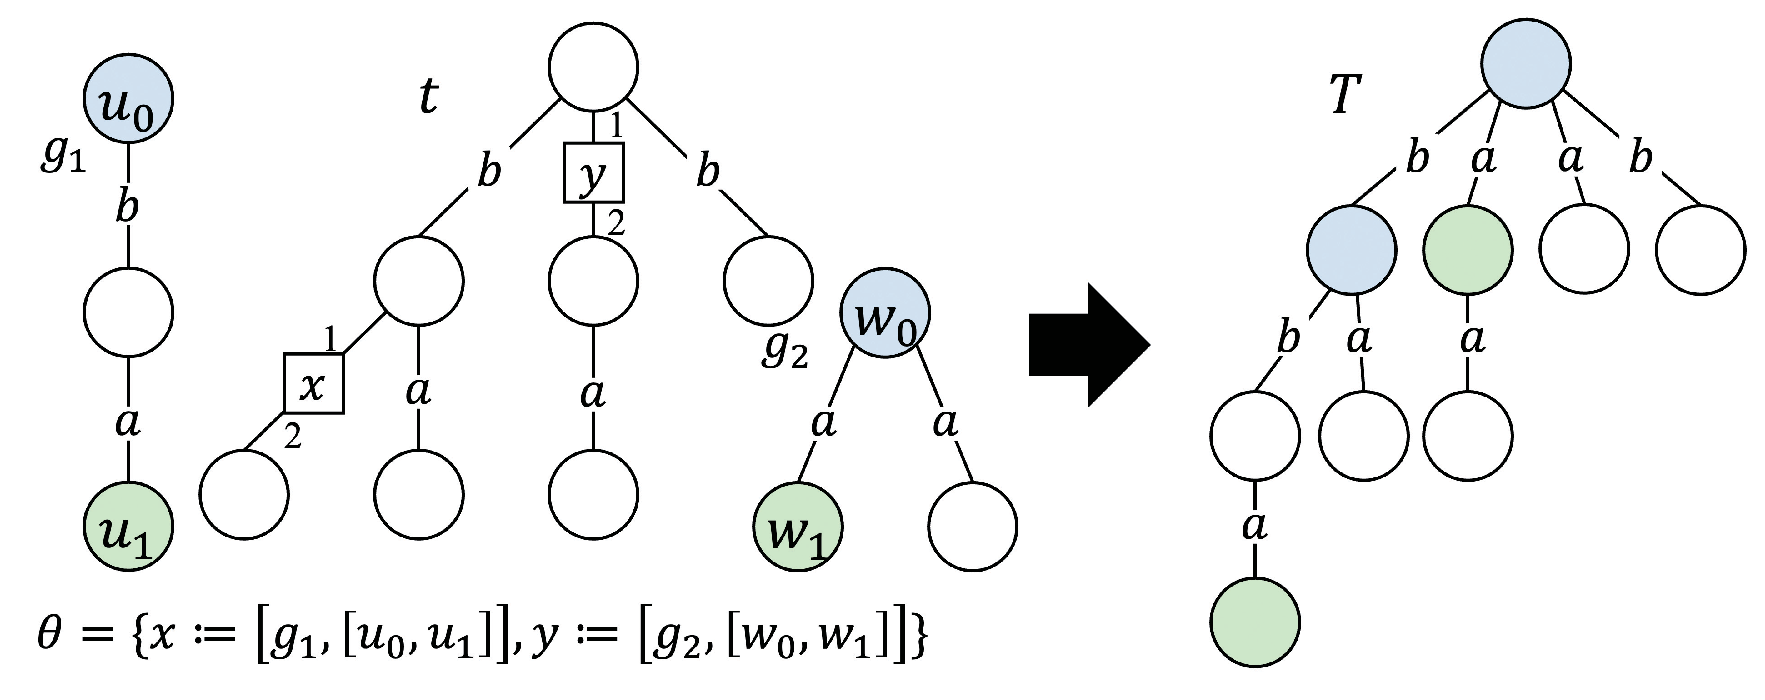
\includegraphics[scale=0.5]{fig-lottp.eps}
  \caption{線形順序項木パターン$t$と順序木$t\theta \equiv T$}\label{fig:lottp}
\end{figure}

% 定義9
\begin{define}{\bf 順序項木パターン言語}\par
  順序項木パターン$t\in {\cal OTTP}_{\Sigma,\Lambda,X}$に対して,$t$の順序項木パターン言語$L(t)\subseteq {\cal OT}_{\Sigma,\Lambda}$を次のように定義する:
  $$L(t)=\{t\theta\in {\cal OT}_{\Sigma,\Lambda}\mid \mbox{$\theta$は$t$の変数への任意の代入}\}.$$

  \noindent
  順序項木パターン$t$に対して,$T\in L(t)$となる順序木$T$の例を図\ref{fig:lottp}にあげる.
\end{define}

線形順序項木パターン$t$と順序木$T$に対して,$t\theta\equiv T$となるような代入$\theta$が存在するとき,$t$は$T$にマッチするという.線形順序項木パターン照合問題は次のように定義される決定問題である:

\medskip
\noindent
\textbf{線形順序項木パターン照合問題}(${\cal LOTTP}$-${\cal MP}$)\\
\textbf{入力}: 線形順序項木パターン$t$と順序木$T$.\\
\textbf{問題}: $t$は$T$にマッチするか?
\medskip

Suzuki et al.\cite{suzuki-tcs2006}は,線形順序項木パターン照合問題を解く$O(nN)$時間逐次アルゴリズムを提案した.$n$と$N$はそれぞれ線形順序項木パターン及び順序木の頂点数である.

% 2.5
% 質問学習モデル
% 2.5
\subsection{質問学習モデル}
質問学習モデルはAngluin\cite{angluin-ml1988}により提案された計算論的学習理論における機械学習モデルの一つである.質問学習モデルにおいては,学習対象に関する質問に正しく答えることができる完全な教師を仮定する.この教師の役割は,現実的には実現するのが難しい状況が多く,その意味で\textbf{オラクル(oracle)}と呼ぶ.学習対象に関する質問に対して,オラクルを仮定して計算量などの解析を行う.

質問学習モデルにおいて最もよく用いられる質問として所属性質問と等価性質問がある.学習対象の概念$C$に関する所属性質問とは「任意に与えられた要素$x$が$C$に属するか否か」を問い,$Yes$か$No$のどちらかで答えを受け取る質問である(図\ref{fig:ql}).等価性質問は,学習の過程で生徒が仮説$G$を見つけたとするとき,「$G$は正しい学習対象$C$と等しいですか?」と問い,もし等しければ$Yes$と,そうでなければその反例をひとつ受け取る質問である.

% 図2.6
\begin{figure}[tb]
  \centering
  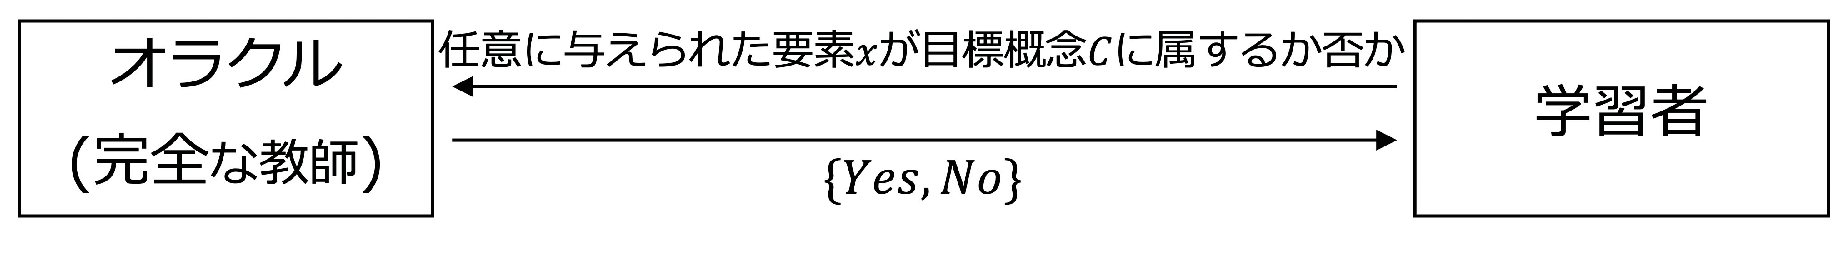
\includegraphics[scale=0.28]{fig-ql.eps}
  \caption{一般に学習対象の概念$C$に関する所属性質問}\label{fig:ql}
\end{figure}
